\documentclass[12pt, oneside]{article}
\usepackage[letterpaper, margin=1in, headsep=0.5in]{geometry}
\usepackage[english]{babel}
\usepackage[utf8]{inputenc}
\usepackage{amsmath}
\usepackage{amsfonts}
\usepackage{amssymb}
\usepackage{tikz}
\usepackage{tkz-fct}
\usepackage{pgfplots}
\pgfplotsset{width=10cm,compat=1.9}
\usepgfplotslibrary{statistics}
\usepackage{pgfplotstable}
%\usepackage{venndiagram}

\usepackage{fancyhdr}
\pagestyle{fancy}
\fancyhf{}
\rhead{\thepage \\Name: \hspace{1.5in}.\\}
\lhead{BECA / Dr. Huson / 11.1 IB Math SL\\* 10 May 2018 \\*\textbf{Test: Statistics, exponential, \& polynomial functions
}}

\renewcommand{\headrulewidth}{0pt}

\begin{document}


%\subsection*{Solve equations}

%Solve for the value of $x$.
\vspace{1cm}

\begin{enumerate}


\item In an arithmetic sequence, the first term is 5 and the second term is 7.
\begin{enumerate}
    \item Find the common difference.
        \begin{flushright}[2]\end{flushright}
    \item Find the tenth term.\\[50pt]
        \begin{flushright}[2]\end{flushright}
    \item Find the sum of the first fifteen terms of the sequence. \\[50pt]
        \begin{flushright}[2]\end{flushright}
\end{enumerate}

\item Simplify the expression $\sqrt{x^4 y^2}$.\\*[50pt]
        \begin{flushright}[2]\end{flushright}

\item Carlos puts \$12,500 into an investment account with interest compounded continuously. If the annual interest rate is 3.15\% what is the balance after 5 years? %\\[80pt]
        \begin{flushright}[5]\end{flushright}

\newpage
\item Given the function $f(x)=x^3-2x^2-5x+6$. 
\begin{enumerate}
    \item Write down the $y$-intercept.
        \begin{flushright}[1]\end{flushright}%\\*[10pt]
    \item Find the $x$-intercepts, rounding to the nearest hundredth.\\*[30pt]
        \begin{flushright}[2]\end{flushright}

    \item Graph the function on the grid below, carefully passing through the correct intercepts. 
        \begin{flushright}[3]\end{flushright}

\end{enumerate}

\begin{figure}[!ht]
    \centering
    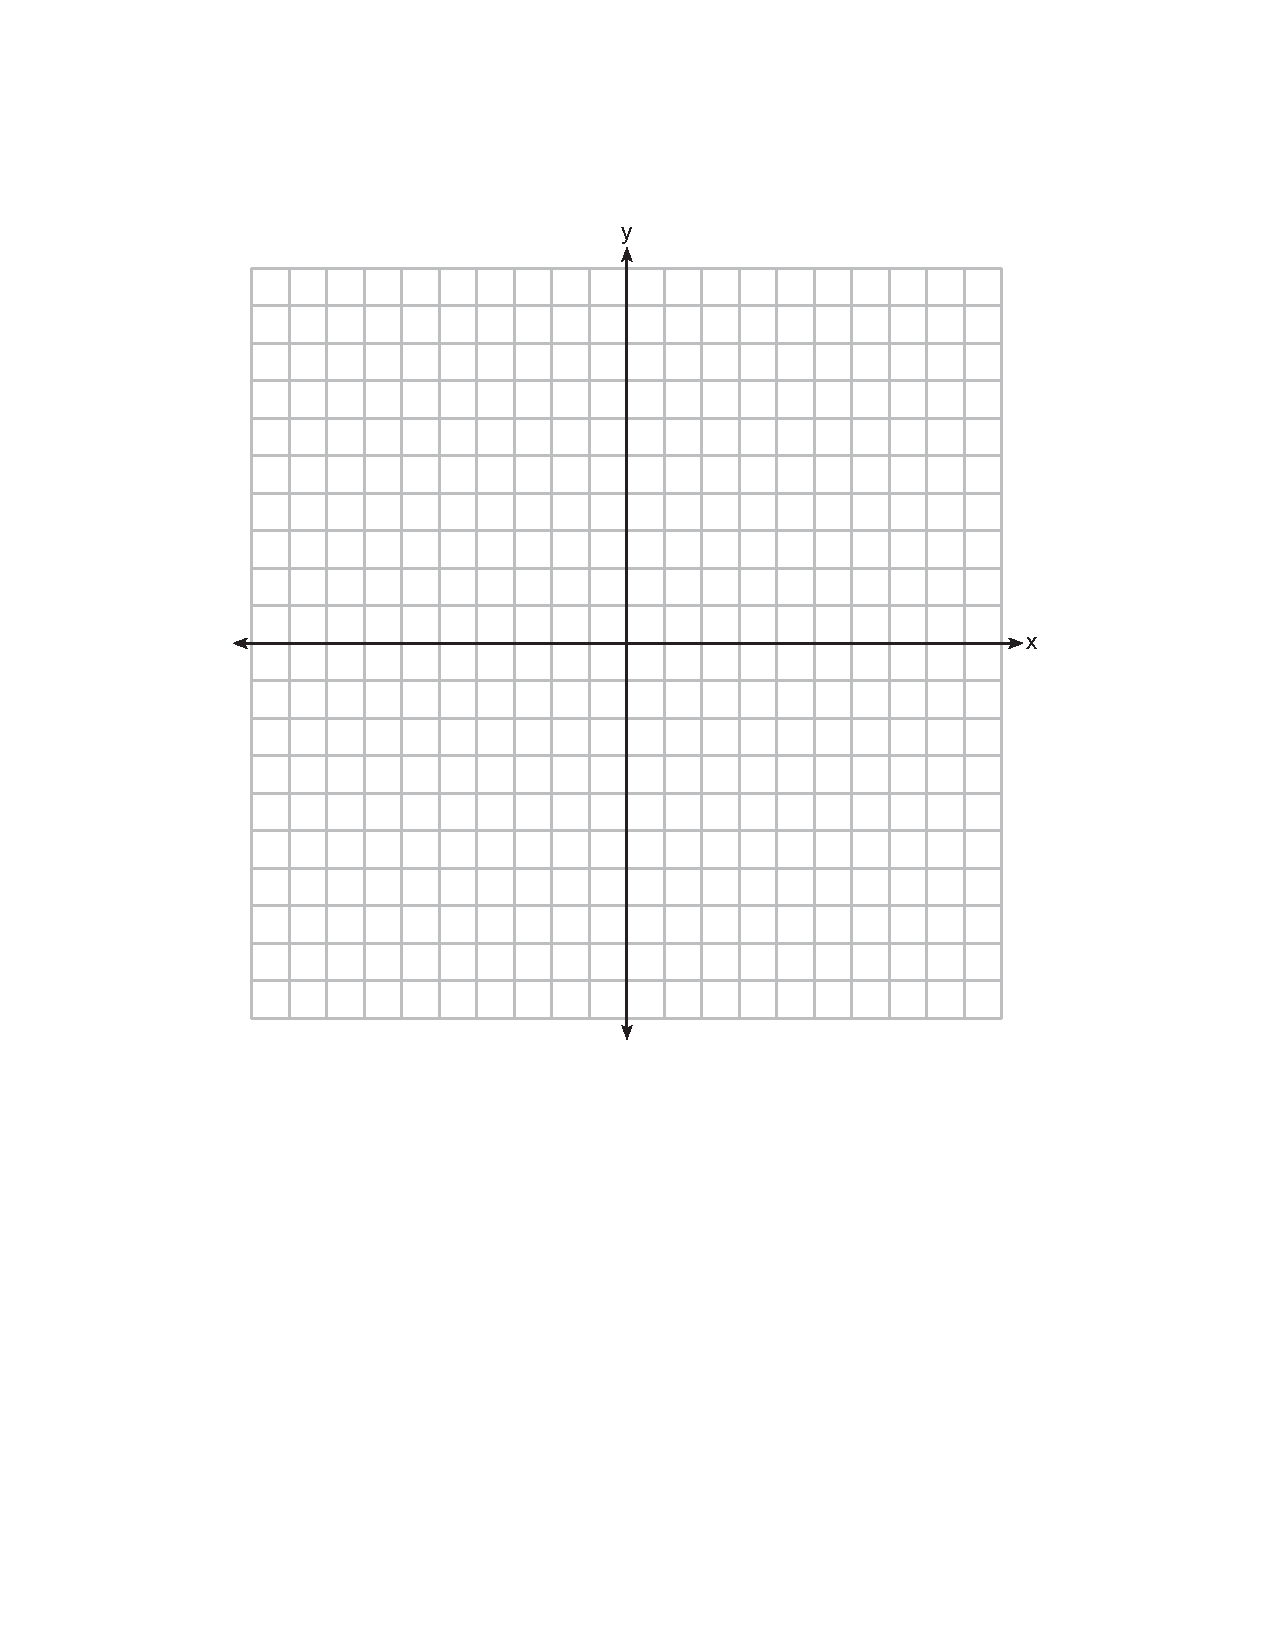
\includegraphics[width=0.75\textwidth]{regents-grid.pdf}
\end{figure}

\newpage

\item The expression $(x + a)(x + b)$ can not be written as
\begin{enumerate}
    \item $a(x + b)+ b(x + b)$
    \item $x^2 + ax + bx + ab$ 
    \item  $x^2 + (a + b)x + ab$  
    \item $x(x + a)+ b(x + a)$
\end{enumerate}
        \begin{flushright}[2]\end{flushright}

\item Consider a geometric sequence where the first term is 138 and the second term is 115.
\begin{enumerate}
    \item Find the common ratio, $r$.\\[20pt]
        \begin{flushright}[1]\end{flushright}
    \item Find the seventh term.\\[80pt]
        \begin{flushright}[2]\end{flushright}
    \item Find the least value of $n$ such that the $n$th term of the sequence is less than 20. \\[80pt]
        \begin{flushright}[3]\end{flushright}
\end{enumerate}

\newpage
\item Algebraically determine the values of $h$ and $k$ to correctly complete the identity stated below.
\[3x^3-5x^2+3=(x-2)(3x^2+hx+2)+k\] \\[2in] 
        \begin{flushright}[4]\end{flushright}

\item Three consecutive terms of a geometric sequence are $x-5$, 8, and $x+7$.\\
Find the possible values of $x$.\\[3in]
    \begin{flushright}[6]\end{flushright}

\newpage
\item A bank account earns interest at a continuous interest rate of 3.925\% per year. The initial deposit is \$175. Which function models the value of the balance? \qquad [2]
\begin{enumerate}
    \item $P(t)=175 \cdot 1.04^{t}$
    \item $P(t)=175 (1+0.03925)^{t}$
    \item $P(t)=175 \cdot 1.03925^{t}$
    \item $P(t)=175 \cdot e^{0.04t}$
\end{enumerate}
    %\begin{flushright}[5]\end{flushright}


\item Write $\sqrt{a^5} \div a^{\frac{1}{2}}$ as an expression with positive, integer exponents.\\*[40pt]
    \begin{flushright}[3]\end{flushright}

\item The function $p(t)=110e^{0.0325t}$ models the population of a city, in millions, $t$ years after 2010.
\begin{enumerate}
    \item Initially, as of 2010, what is the population in millions?%\\[20pt]
        \begin{flushright}[1]\end{flushright}
    \item What is the annual continuous rate, expressed as in percent, that the population increases?%\\[10pt]
        \begin{flushright}[1]\end{flushright}
    \item Find the population in 2015, rounded to the nearest million.\\[60pt]
        \begin{flushright}[2]\end{flushright}
    \item In what year will the population be approximately 138 million?
        \begin{flushright}[2]\end{flushright}
\end{enumerate}



\end{enumerate}
\end{document}